\documentclass[10pt,twocolumn,letterpaper]{article}

\usepackage{cvpr}
\usepackage{times}
\usepackage{epsfig}
\usepackage{graphicx}
\usepackage{amsmath}
\usepackage{amssymb}


\newcommand\myworries[1]{\textcolor{red}{#1}}
% Include other packages here, before hyperref.

% If you comment hyperref and then uncomment it, you should delete
% egpaper.aux before re-running latex.  (Or just hit 'q' on the first latex
% run, let it finish, and you should be clear).
\usepackage[breaklinks=true,bookmarks=false]{hyperref}

\cvprfinalcopy % *** Uncomment this line for the final submission

\def\cvprPaperID{****} % *** Enter the CVPR Paper ID here
\def\httilde{\mbox{\tt\raisebox{-.5ex}{\symbol{126}}}}

% Pages are numbered in submission mode, and unnumbered in camera-ready
%\ifcvprfinal\pagestyle{empty}\fi
\setcounter{page}{1}
\begin{document}

%%%%%%%%% TITLE
\title{3D Object Detection and Tracking using Graph Neural Networks on Waymo Dataset}

\author{Ahmed Bahnasy\\
Technical University in Munich\\

{\tt\small ahmed.bahnasy@tum.de}
% For a paper whose authors are all at the same institution,
% omit the following lines up until the closing ``}''.
% Additional authors and addresses can be added with ``\and'',
% just like the second author.
% To save space, use either the email address or home page, not both
}

\maketitle
%\thispagestyle{empty}

%%%%%%%%% ABSTRACT
\begin{abstract}
Recent approaches for 3D object detection have made a tremendous progress due to the development of deep learning. this also highly influences the  progress in other tasks like 3D Multi-object tracking (MOT) which is an indispensable component to any autonomous system. Recent work uses a standard tracking- by-detection pipeline, where feature extraction is first per- formed independently for each object in order to compute an affinity matrix. Then the affinity matrix is passed to the Hungarian algorithm for data association. This matching can be seen as discrete optimisation process and there is no learning it. A key factor of this standard pipeline is to learn discriminative features for different objects, by relying on a robust detector in order to reduce confusion during data association. In this task, we experiment with improving the discriminative feature learning for MOT: by first build a robust object detector and second instead of obtaining features for each object independently, we try applying learning module for tracking by introducing the Graph Neural Network which enables feature interaction mechanism. As a result, the feature of one object is informed of the features of other objects so that the object feature can lean towards the object with similar feature (i.e., object probably with a same ID) and deviate from objects with dissimilar features (i.e., object prob- ably with different IDs), leading to a more discriminative feature for each object
\end{abstract}

%%%%%%%%% BODY TEXT
\section{Introduction}

\paragraph{}
Robust 3D perception becomes an essential component in any state-of-the-art autonomous system. 3D detection has a series of challenges: First, point-clouds are sparse, the points are unevenly distributed across the 3D space, and most of the 3D space are without measurements. Second, 3D objects have a wide range of sizes, shapes and aspect ratios, for example, in autonomous driving domain, buses, trucks and cars are elongated, pedestrians are tall and cyclists are nearly planer. These challenges makes applying ideas from 2D domain to 3D domain not straight forward. trying to use the anchor based approach followed in 2D domain by assigning a different anchor for each object orientation increases the computational cost and may introduce a large number of of potential false-positive detections. the main challenge for linking up 2D and 3D domains lies in the way the objects are represented \cite{yang20203dssd}. representing objects as points greatly simplifies 3D recognition \cite{yin2020center}. In this task, we tried to build a 3D that detects centers of the objects and their properties using a key-point detector \cite{zhou2019objects}. In specific we followed the same approach in \cite{yin2020center, ge2020afdet} by using any standard Lidar-based backbone network, for example, PointPillars or VoxelNet, to build an intermediate representation for the input point cloud. this representation is then flattened into Birds-Eye-View map using a standard image-based key-point detector to find object centers \cite{zhou2019objects}. the rest of the 3D bounding box parameters, i.e., 3D Size, orientation, and velocity, are then regressed from the center location vector. according to \cite{yin2020center}, center-based representation has several advantages: First, it reduces the detector search space since points has no orientation, unlike bounding boxes. Second, center-based representation simplifies the tracking downstream tasks. 

\paragraph{}
Much like 3D perception, Multi-object tracking (MOT) is a crucial component for autonomous driving \cite{luo2018fast}. Tracking-by-detection paradigm is the dominant approach when it comes to online MOT problems \cite{bewley2016simple, weng2019baseline}. The main idea is to apply object detector to all frames and extract features independently from each detected object. Then pairwise similarity is computed between objects and a Hungarian algorithm \cite{kuhn1955hungarian} is used to solve the problem. The key idea in this approach is to learn discriminative features for the objects with different identities to reduce the confusion in the matching. One key observation is that feature extraction is done independently and there is no interaction between features during feature extraction. according to \cite{weng2020gnn3dmot}, independent feature extraction is sub-optimal for discriminative feature learning. this idea is very important for MOT, given the fact that an object in current frame can be matched to at most one object in the previous frame. so if the similarity between two features increased, then the pairwise similarity between the rest of the objects and any of these two objects should be decreased to avoid confusion for matching. based on that observation, we followed \cite{weng2020gnn3dmot} by implementing a Graph Neural Network to do the feature interaction. The idea is to construct a graph with each node being the object feature. Then, each node can update its feature by aggregating features from other nodes during layer propagation step. the object feature is now not isolated and can be adapted with respect to other features.

\myworries{state the achievements and the results of the work with numbers !}
%-------------------------------------------------------------------------

\section{Related Work}

\paragraph{3D Object Detection} is all about predicting the three dimensional rotated bounding boxes \cite{geiger2012we, lang2019pointpillars, qi2018frustum, yan2018second, yang20203dssd, yang2019std}. Most 3D-based methods either use point cloud data directly or require converting these data into 3D grids or voxels instead of generating BEV representations. In \cite{wang2015voting}, point cloud data are converted into voxels containing feature vectors, and then a novel convolution-like voting-based algorithm is used for detection. Vote3Deep \cite{engelcke2017vote3deep} leverages feature voting in \cite{wang2015voting} to efficiently process the sparse 3D point-cloud in equally spaced 3D voxels. VoxelNet \cite{zhou2018voxelnet} uses a PointNet \cite{qi2017pointnet} inside each voxel to generate a unified feature representation from which a head with 3D sparse convolutions \cite{graham20183d} and 2D convolutions produces detections. SECOND \cite{yan2018second} simplifies the VoxelNet and speeds up sparse 3D convolutions. PIXOR \cite{yang2018pixor} project all points onto a 2D feature map with 3D occupancy and point intensity information to remove the expensive 3D convolutions. PointPillars\cite{lang2019pointpillars} replaces all voxel computation with a pillar representation, a single tall elongated voxel per map location, improving backbone efficiency. MVF \cite{zhou2020end} and Pillar-od \cite{wang2020pillar} combine multiple view features to learn a more effective pillar representation. In this task we followed \cite{yin2020center, ge2020afdet} by focusing on the output representation and employ any 3D encoder to get the representation.

\paragraph{Online Multi-Object Tracking} is mostly addressed using Tracking by Detection paradigm. the performance is highly impacted by two factors: object detection quality and discriminative feature learning. After the affinity matrix is computed based on the pairwise similarity of learned discriminative feature, the problem of online MOT could be addressed as as a discrete optimization problem and could be solved using as  bipartite matching problem using the Hungarian algorithm \cite{kuhn1955hungarian}. To obtain discriminative feature, prior work mostly focuses on the feature selection. Among different features, it turns out that motion and appearance are the most dis- criminative features. Early work employs hand-crafted features such as spatial distance \cite{pirsiavash2011globally} and Intersection of Union (IoU) \cite{bochinski2017high} as the motion feature, and use color histograms as the appearance feature. Recently, Convolutional Neural Networks have been used to extract appearance feature \cite{baser2019fantrack, frossard2018end}. Regarding the motion feature, many filter based approaches has been used \cite{bewley2016simple, weng2019baseline}. Deep learning approaches has been introduced for motion feature in \cite{baser2019fantrack}. we followed the same idea in \cite{wojke2017simple, weng2020gnn3dmot} by exploring both the appearance and motion feature with focus on the 3D space.

\paragraph{Graph Neural Networks} is used as way to improve discriminative feature learning for MOT after showing promising performance in many fields\cite{hamilton2017inductive,velivckovic2017graph,kipf2016semi, berg2017graph, monti2017geometric, ying2018graph}. GNNs was first proposed by \cite{gori2005new} to directly process graph-structured data using neural networks. The major component of the GNNs is the node feature aggregation technique, with which node can update its feature by interacting with other nodes. With this technique, significant success has been achieved in many fields using GNNs such as semantic segmentation\cite{chen2019graph}, action recognition \cite{shi2019skeleton}, single object tracking \cite{gao2019graph}, person re-identification \cite{wu2019unsupervised}, point cloud classification and segmentation \cite{wang2019dynamic}. The majority of the work deals with object features as independent and isolated from other features. by leveraging node aggregation technique of the GNNs, object features could be iteratively evolved so that the feature of different objects can be more discriminative. the idea of feature interaction was first introduced in \cite{hu2018relation} to encode context information for object detection in the spatial domain, Although a temporal relation network is proposed in the follow-up work \cite{xu2019spatial}, the feature of a tracked object is only aggregating from its past trajectory and no interaction with other object features exist. in This task we followed \cite{yin2020center} by implementing a generic feature interaction framework that can model any kind of interaction in both spatial and temporal domains



%-------------------------------------------------------------------------

\section{Network Architecture}

During the early stages of this task, we tried to use Votenet \cite{qi2019deep} as a 3D object detector. Despite the promising results of this architecture on Indoor dataset, it performs very poorly on outdoor datasets like KITTI and Waymo. More information about these experiments are stated Appendix \ref{appendix:votenet}

\subsection{Detection}

\paragraph{Point Cloud Encoder.} We followed the same approach of up to date SOTA detectors \cite{sota on waymo} on Waymo dataset\cite{dataset} by, first, employing a 3D encoder that quantizes the point-cloud into regular bins. A point-based network then extracts feature for all points inside a bin. The 3D encoder then pools these features into its primary feature representation. Second, the output of the encoder is processed by a backbone network. The output of a backbone network is a map-view feature-map  \textbf{M}  $ \in \mathbb{R}^{W \times L\times F}$ of width $W$ and length $L$ with $F$ channels in a map-view reference frame. Both width and height directly relate to the resolution of individual voxel bins and the backbone network’s stride. Common Common backbones used for this task are VoxelNet \cite{second, pixor} and PointPillars \cite{PointPillars}. A number of separate heads modules take the feature-map \textbf{M} and predict a class-specific heat-map, object size, a sub-voxel location refinement, rotation, and velocity. All outputs are dense predictions. Figure \ref{fig:detection_network} shows the overall Detection Network.

\begin{figure*}
	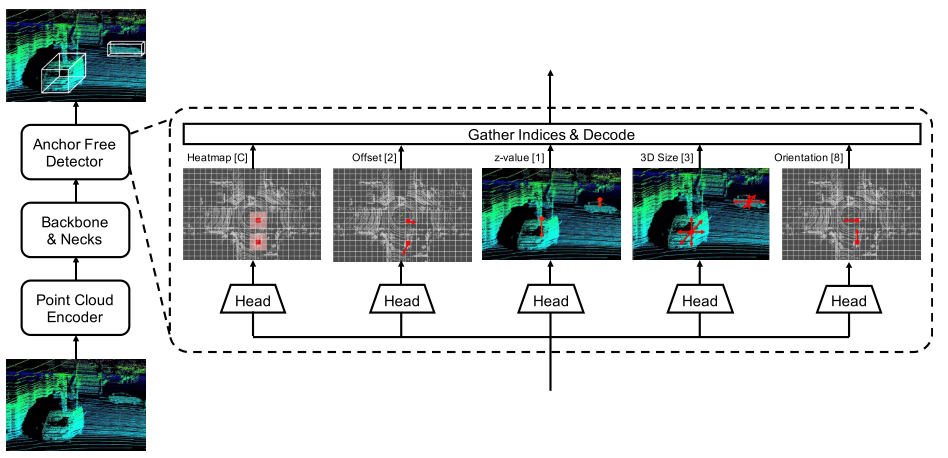
\includegraphics[width=\linewidth]{media/detection_net.png}
   \caption{Overall Architecture of the Detection Network. source \cite{ge2020afdet}}
\label{fig:detection_network}
\end{figure*}

\paragraph{Center heatmap head.}
This head produces a heatmap peak at the center location of any detected object. This head produces a K-channel heatmap $\hat{Y}$, one channel for each of K classes. During training, it targets a 2D Gaussian produced by the projection of 3D centers of annotated bounding boxes into the map-view. Following \cite{zhou2019objects}, a focal loss is used.

\paragraph{Regression heads.}
Several object properties are stored at the center-features of the objects: sub-voxel refinement $o \in \mathbb{R}^{2}$, height above the ground $h_{g} \in \mathbb{R}$, the 3D size $s \ in \mathbb{R}^{3}$, and a heading rotation angle $(\sin{(\alpha)}, \cos{(\alpha)}) \in \mathbb{R}^{2}$. Sub-voxel refinement is meant to reduce the quantization error. Heading prediction uses the sine and cosine of the heading angle as a continuous regression target.

\subsection{Tracking}
Given $M$ tracked objects $o_{i} \in O$ at frame $t$ where $i \in {1,2,..., M}$ and $N$ detected objects $d_{j} \in D$ in frame $t+1$ where $j \in {1,2,...,N}$, the idea of MOT is all about associating existing tracked objects $M$ from previous frame $t$ with new detected objects $N$ in the current frame $t+1$ by learning discriminative feature from $O$ and $D$ and then find the correct matching based on the pairwise feature similarity.

Following \cite{weng2020gnn3dmot}, we implemented a 3D appearance extractor and 3D motion extractor which are both applied to all objects in $O$ and $D$ and then the concatenated together. A graph neural network is then implemented that takes as input the concatenated object and construct a graph with node being the object feature in frame $t$ and $t+1$. Then, the graph neural network iteratively aggregates the node feature from the neighbourhood and computes the affinity matrix for matching using edge regression. Following the \cite{shi2019pointrcnn}, the 3D detection is parametrized as a tuple of $d = {x,y,z,l,w,h,\theta}$ where $(x,y,z)$ denotes the object center in 3D space, $(l,w,h)$ denotes the object size and $\theta$ is the heading angle. The tracked objects $O$ use the same parametrization alongside an additional ID. the feature extractors are depicted in Figure \ref{fig:tracking_feature_ext}.

\begin{figure}
	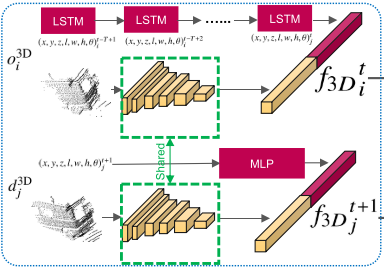
\includegraphics[width=\linewidth]{media/tracking_net.png}
   \caption{source \cite{weng2020gnn3dmot}}
\label{fig:tracking_feature_ext}
\end{figure}

\subsubsection{Feature Extractor}

For appearance feature extractor, LiDAR point cloud as used as the appearance cue. the point cloud enclosed by the 3D detection box is extracted and then PointNet \cite{pointnet} is applied to obtain the feature. The same appearance feature extractor is applied on both the tracked and the detected objects. For the motion feature extractor, different methods are used. for tracked objects, they have temporal data in form of an associated trajectory in the past frames. while detected objects do not have. for Tracked objects $o_{i}$, an LSTM is used to take as input the object\'s detections in the past T frames to obtain the feature. For detected object $d_{j}$, Two-Layer MLP (Multi-Layer-perceptron) is used that takes the detection in frame $t+1$ as input to extract the feature. The final feature for tracked and detected objects is obtained by concatenating the 3D motion and appearance features. The final motion and appearance vectors are adjusted to have the same dimensionality to ensure fair contribution for both features in the final representation of the object.



\subsubsection{Graph Neural Network for Data Association}

\paragraph{Graph Construction.}
After feature extraction, we end up with M features for tracked objects in frame t and N features for detected objects in frame t+1. A graph, of total nodes N+M, is constructed with each node being an object feature. an important step is to define the neighbourhood for every node in the graph. A naiive approach is to make it fully connected. The downside of this approach is the computational complexity. Based on the prior knowledge about online MOT, where the matching should be done across frames and the possible matching should be done with only nearby frames, the edges are constructed between pairs of nodes in different frames and only if the distance between their detection centers is less than $Dist_{max}$.

\paragraph{Affinity Matrix using Edge Regression.}
an $NxM$ is needed for solving the online MOT.  the affinity matrix is constructed based on the pairwise similarity of the features extracted from $M$ tracked objects and $N$ detected objects. This process is called Edge Regression in context of GNN. Conventional metrics used in MOT community are cosine similarity and negative L2 distance between features pairs. Following \cite{weng2020gnn3dmot}, we implemented a learnable regression module by employing a two-layer MLP that takes the difference of two node features as input and outpus a scaler value between 0 and 1 as the pairwise similarity score: 
\begin{equation}
A_{ij} = Sigmoid(\sigma_{2}(ReLU(\sigma_{1}(n^{t}_{i} - n^{t+1}_{j}))))
\end{equation}
where $\sigma_{1}$ and $\sigma_{2}$ are two different linear layers. In addition, $n^{t}_{i}$ and $n^{t+1}_{j}$ are two node features in different frames where $j, i \in {1, 2, ···, M}, j \in {1, 2, ···, N}$
\paragraph{Node feature Aggregation.} The heart of GNN is aggregation step which model the feature interaction. it iteratively update the node feature by aggregating features from the node neighbourhood in every layer of the GNN. Among the vast aggregation rules in the literature, we choose four rules to analyze their impact on the performance of MOT.

The first type is applying general message passing scheme, the second type is using GraphConv operator \cite{}, the third type is using EdgeConv operator \cite{} and the fourth type is using Graph attention mechanism \cite{}

\begin{equation}\label{eq:two}
\acute{n^{t}_{i}} = \sum_{j \in \mathcal{N}(i)} \sigma(ReLU(n^{t+1}_{i}))
\end{equation}
\begin{equation}\label{eq:three}
\acute{n^{t}_{i}} = \sigma_{4}(ReLU(n^{t}_{i})) +  \sum_{j \in \mathcal{N}(i)} \sigma(ReLU(n^{t+1}_{i}))
\end{equation}
\begin{equation}\label{eq:four}
\acute{n^{t}_{i}} = \sigma_{4}(ReLU(n^{t}_{i})) +  \sum_{j \in \mathcal{N}(i)} \sigma(ReLU(n^{t+1}_{i} - n^{t}_{i}))
\end{equation}
\begin{equation}\label{eq:five}
\acute{n^{t}_{i}} = \sigma_{4}(ReLU(n^{t}_{i})) +  \sum_{j \in \mathcal{N}(i)} \sigma(ReLU(A_{ij}(n^{t+1}_{i} - n^{t}_{i})))
\end{equation}

where $\mathcal{N}(i)$ is a set of neighbourhood nodes in frame $t+1$ with respect to the node $i$ in frame $t$. $\sigma_{3}, \sigma_{4}$ are linear layers which have different weights across layers of the GNN. The weight $A_{ij}$ is obtained from the affinity matrix of the current layer. \\
In Eq. \ref{eq:two}, node feature us update by aggregating feature from only the neighbourhood nodes, the node feature itself is lost after aggregation. In Eq. \ref{eq:three}, the previous limitation is addressed by adding self loops in the graph to consider node feature during aggregation. In Eq \ref{eq:four}, feature from neighbourhood is replaced with the difference of the features between the node itself and the neighbourhood node. In Eq. \ref{eq:five}, attention weight is added from the affinity matrix to the feature aggregation so that the network can focus on the neighbourhood with higher affinity score.

\subsubsection{Losses}
Following \cite{weng2020gnn3dmot}, two losses are implemented and used in all K graph layers during the training. The first loss is the batch triplet loss $L_{tri}$, and the second loss is affinity Loss $L_{aff}$. The entire loss function $L$: 

\begin{equation}
L = \sum^{K-1}_{K=0}(L^{k}_{tri} + L^{k}_{aff})
\end{equation}

\paragraph{Bath Triplet Loss.} Applying Batch Triplet Loss to node feature in every layer of the GNN is needed for learning discriminative features for matching. for node $n^{t}_{i}$ that has a matched node in $n^{t+1}_{j}$, the batch triplet loss in each layer is:

\begin{multline}
L_{tri} =  \max(\left\|n^{t}_{i} - n^{t+1}_{j}\right\| - \min_{\substack{\text{$d_{s}\in D$} \\ \text{$id_{i} \neq id_{s}$}}}
{\left\|n^{t}_{i} - n^{t+1}_{j}\right\|} -\\ \min_{\substack{\text{$o_{r} \in O$} \\ \text{$id_{r} \neq id_{j}$}}}{\left\| n^{t}_{i} - n^{t+1}_{j}\right\|}+ \alpha, 0)
\end{multline}
where $\alpha$ is the margin of the triplet loss. $n^{t+1}_{s}$ is a node in frame $t+1$ that has a different ID from node $n^{t+1}_{j}$ and $n^{t}_{i}$. Similarly, $n^{t}_{i}$ and $n^{t+1}_{j}$. In the case that $n^{t}_{i}$ does not have a matched node in frame $t+1$ with the same ID,  the first is deleted for the positive pair and only the remaining two negative terms in the loss are considered.

\paragraph{Affinity Loss.} Additional affinity loss $L_{aff}$ is applied to supervise the final output of the network, i.e., the predicted affinity matrix $A$. The affinity loss consists of two parts and represented as follows: 

\begin{equation}
L_{aff} = L_{bce} + L_{ce}
\end{equation}

First, since the ground truth affinity matrix $A^{g}$ can only have integer 0 or 1 in all the entries, the prediction can be formulated as a classification problem. The first part could be represented as a binary cross entropy loss $L_{bce}$ that is applied on each entry of the predicted affinity matrix $A$.
\begin{equation}
L_{bce} = \frac{-1}{MN}\sum^{M}_{i}\sum^{N}_{j}(A^{g}_{ij} \log A_{ij} +(1-A^{g}_{ij})\log(1-A_{ij}))
\end{equation}

Second, each tracked object $o^{t}_{i}$ in frame $t$ can only have either one matched detection $d^{t+1}_{j}$ or no match at all. Thus, each row and column of the $A^{g}$ can only be a one-hot vector or an all-zero vector. For all rows and columns that have a none-hot vector in $A^{g}$, cross entropy loss $L_{ce}$ is applied. For example, the column $A^{g}_{j}$ in ground truth affinity matrix is a one-hot vector and the loss $L_{ce}$ for the jth column is:
\begin{equation}
L_{ce} = \frac{-1}{M}\sum^{M}_{i} A^{g}_{ij}\log(\frac{\exp{A_{ij}}}{\sum^{M}_{i}\exp{A_{ij}}})
\end{equation}



%-------------------------------------------------------------------------

\section{Experiments}
layers of graphs
different aggregation rules
effect of motion and appearance feature extractors
compare to the baseline model

\subsection{Waymo Dataset.} Waymo Open Dataset \cite{} contains 798 training sequences and 202 validation sequences. it has 5 classes, among them 3 dynamic (moving) classes (Vehicles, Pedesterians, Cyclists) which we consider in our experiments. The point clouds are captured with a 64 lanes LiDAR, which produces about 180k LiDAR points every 0.1s. The official 3D detection evaluation metrics include the standard 3D bounding box mean average precision (mAP) and mAP weighted by heading accuracy (mAPH). we present our results based on mAP only.  The mAP is based on an IoU threshold of 0.7 for vehicles and 0.5 for pedestrians. For 3D tracking, the official metrics are Multiple Object Tracking Accuracy (MOTA) and Multiple Object Tracking Precision (MOTP). We present our results based on MOTA only. The official evaluation toolkit also provides a performance breakdown for two difficulty levels: LEVEL 1 for boxes with more than five Lidar points, and LEVEL 2 for boxes with at least one LiDAR point.
\subsection{Data Augmentation}
For data augmentation, we use random flipping along both X and Y axis, and global scaling with a random factor from [0.95, 1.05]. We use a random global rotation between [$ -\pi/4, \pi/4$]. We also use the ground-truth sampling \cite{yan2018second} to deal with the long tail class distribution, which copies and pastes points inside an annotated box from one frame to another frame. We train the model with batch size of 4 for 20 epochs on GTX1070 ti GPU.

\myworries{mention in this section also the sampler, mention an ablation study showing difference between class weights vs sampler}
\subsection{Implementation Details}

\paragraph{Detector.} The implemented detection model uses a detection range of [$-$75.2m, 75.2m] for the X and Y axis, and [$-$2m, 4m] for the Z axis. Following \cite{cite PV-RCNN}, Voxel size is (0.1m, 0.1m, 0.15m). We followed \cite{yan2018second, yin2020center} by replacing the expensive 3D convolutional middle layers by sparse convolutions \cite{graham20183d}. All heads outputs share a first $3 \times 3$ convolutional layer, Batch Normalization, and ReLU. Then, each output uses its own branch of two $3\times 3$ convolutions separated by a batch norm and ReLU.

\paragraph{Tracker.} Both appearance extractor and motion extractor feature vector dimensionality is set to 128. For appearance branch, PointNet is used with six 1D Convolutional layers that maps the input point cloud with size of $N \times 5$ to $N \times 128$. Then a max pooling operation is applied along the points features to obtain the final appearance feature with dimensionality of 128. for motion feature, two layer LSTM with a hidden size of 128 and number of past frames T=5 is used for tracked objects. For detected objects, two-layer MLP (7, 64,128) is used. a max distance $Dist_{max}=5$ is set to define the neighbourhood for constructing the graph. four graph layers, each with the same dimensionality of 256 are used. For edge regression, two-layer MLP with hidden feature dimension (256,64,1) is used. the margin value $\alpha$ for the batch triplet loss is set to 10.


\paragraph{Tracking Baseline.} A velocity-based closest distance matching, which doesn't require separate model motion, is used as a baseline. it is based on the velocity predictions of the detected objects. it predicts the difference in object position between the current and the past frame. At inference time, the object centers in the current frame are projected back to the previous frame by applying the negative velocity estimate and then matching to the tracked objects is done in a greedy way by closest distance matching.
\myworries{Check also baseline tracker mentioned in Waymo Paper and see if it could be used for comparison, even comparing the numbers without implementation}

\subsection{Main Results}
we show per class comparisons with the state-of-the-art methods in table \ref{tab:waymo_det_sota} \myworries{fill the table !}

\begin{table}
\begin{center}
\begin{tabular}{|l c c c c|}
\hline
Model & mAP & Vehicle & Pedestrian & Cyclists \\
\hline\hline
SA1 (PC) & x & 2048  \\
SA2 (SA1) & x & 1024  \\
SA3 (SA2) & x & 512  \\
SA4 (SA3) & x & 256  \\
FC1 (SA3, SA4) & x & -  \\
FC2 (SA2, SA3) & x & -  \\
\hline
\end{tabular}
\end{center}
\caption{Comparison with some state-of-the-art. the table shows mAP and mAP for each class}
\label{tab:waymo_det_sota}
\end{table}


\subsection{Ablation Study}

\paragraph{Augmentations.} we show the impact of some augmentations in \ref{tab:detection_ablation}
\myworries{mention class reweighting}

\paragraph{anchor vs point based approaches}

\begin{table}
\begin{center}
\begin{tabular}{|l c|}
\hline
Method & mAP \\
\hline\hline
Baseline & 2048  \\
+ GT Sampler & 1024  \\
+ Rotation & 512  \\
+ Filter Empty Boxes & 256  \\
\hline
\end{tabular}
\end{center}
\caption{Ablation studies for Detection}
\label{tab:detection_ablation}
\end{table}

\paragraph{Feature Extractor}
Table \ref{tab:feat_extractor} shows the effect of each individual feature extractor and the combination between them. it is obvious from the results that combining both improves the performance.

\begin{table}
\begin{center}
\begin{tabular}{|l c|}
\hline
Extractor & MOTA (\%) $\uparrow$ \\
\hline\hline
A & 2048  \\
M & 1024  \\
A+M  & 512  \\
\hline
\end{tabular}
\end{center}
\caption{Effect of feature extractors: A (appearance), M (motion)}
\label{tab:feat_extractor}
\end{table}

\paragraph{Number of layers}
\myworries{Plot a graph here !}

\paragraph{Node Aggregation.}

Table \ref{tab:node_aggregator} shows the effect of different node aggregators

\begin{table}
\begin{center}
\begin{tabular}{|l c|}
\hline
Node Aggregation & MOTA (\%) $\uparrow$ \\
\hline\hline
Mean aggregator & 2048  \\
GCN \cite{kipf2016semi}& 1024  \\
SAGEConv \cite{hamilton2017inductive} & 512  \\
GATConv \cite{velivckovic2017graph}  & 512  \\
AGNNConv \cite{thekumparampil2018attention}  & 512  \\
EDGEConv  \cite{wang2019dynamic} & 512  \\
\hline
\end{tabular}
\end{center}
\caption{Effect of different Node aggregators}
\label{tab:node_aggregator}
\end{table}



{\small
\bibliographystyle{ieee_fullname}
\bibliography{egbib}
}


\appendix
\section*{Appendices}
\addcontentsline{toc}{section}{Appendices}
\renewcommand{\thesubsection}{\Alph{subsection}}

\subsection{Votenet for Lidar Outdoor Scenes}\label{appendix:votenet}

\subsubsection {Data preparation and Training}
VoteNet consists of two modules: the proposal module which consumes the raw point cloud and produces the virtual voting points; and the object proposal and classification module that operates on the voting points to propose and classify objects. Up to now, VoteNet has only been tuned and tested on RGB-D data (ScanNet and SUN RGB-D). in order to adapt the model for Waymo, we implemented a custom input pipeline to optimally preprocess and feed the Waymo point cloud data into the VoteNet network.
Following the same train/validation/test split from Waymo paper \cite{cite waymo}, and following the same training procedure mentioned in \cite{votenet}, For each scene we randomly subsample 20k points. The scenes are furthermore augmented on-the-fly with random flips in horizontal plane, random uniform rotations along up-axis in  $\pm$30$^{\circ}$ range, and random uniform scaling of $\pm$10\%. In addition to three Euclidean coordinates for each point, we also include up to two additional features: the provided laser reflection intensities, and a height estimate for each point. The latter is estimated as a 1\% percentile of all point positions along the up-axis.
We perform training on the dynamic classes of the Waymo dataset: car, pedestrian, and cyclist. We choose one size template per class, and 12 bins for the heading angle. We train with a batch size of 16 and incorporate a scheduled learning policy with a starting LR of 0.001 and LR-decays by 0.1 at 60, 90, and 120 epochs, as well as an exponential BN momentum decay. We use same loss function as in SUN RGB-D case.
\paragraph{}
Points clouds from outdoor LiDAR scans are quite different from point clouds from RGB-D indoor scans. For example, the typical scales of the Waymo scenes are significantly larger than those of indoor scans, with depth fields reaching beyond 70 meters along forward-axis. the LiDAR point cloud has strongly varying density and is generally more sparse than the point clouds produced from the RGB-D imagery. Point features extracted from sparse regions may generalize poorly to dense regions, and vice versa

to further adapt VoteNet to the distinct characteristics of the outdoor LiDAR scenes. we adapt the receptive field radii and increase the number of clusters for feature aggregation. to capture fine details of point cloud and, at the same time, mitigate  the corruption of local patterns due to sampling deficiency in sparse cloud regions, we enhance the set-abstraction modules of the backbone network with multi-scale grouping (MSG) layers \cite{pointnet++}, which concatenate features at different scales before feeding them into the feature aggregation layer.

Among all the experiments to find the best backbone network parameters, we ended up following the configuration in \cite{RCNN paper} by configuring four MSG-based SA layers used to subsample the inputs to 4096, 1024, 256 and 64 points, and two FP layers to upsample the points back to 1024 points, each with additional 512 deep features. Tables \ref{tab:votenet_oringinal} and \ref{tab:votenet_msg} illustrates the difference between the two backbones.


\begin{table*}
\label{tab:votenet_oringinal}
\begin{center}
\begin{tabular}{|c|c|c|c|c|}
\hline
Module (Input) & Output dimensions & clusters K & Receptive field radius & MLP layer dimensions \\
\hline\hline
SA1 (PC) & (4096, 3 + 96) & 2048 & 0.2 & 64/64/128 \\
SA2 (SA1) & (1024, 3 + 256) & 1024 & 0.4 & 128/128/256 \\
SA3 (SA2) & (512, 3 + 512) & 512 & 0.8 & 128/128/256 \\
SA4 (SA3) & (64, 3 + 512) & 256 & 1.2 & 128/128/256 \\
FC1 (SA3, SA4) & (512, 3 + 512) & - & - & 512/512 \\
FC2 (SA2, SA3) & (1024, 3 + 512) & - & - & 512/512 \\
\hline
\end{tabular}
\end{center}
\caption{Original Architecture of VPN in \cite{votenet paper}}
\end{table*}



\begin{table*}
\label{tab:votenet_msg}
\begin{center}
\begin{tabular}{|c|c|c|c|c|}
\hline
Module (Input) & Output dimensions & clusters K & MSG Radii & MLP layers \\
\hline\hline
SA1 (PC) & (4096, 3 + 96) & 2048 & 0.1,  0.5 & 16/16/32, 32/32/64 \\
SA2 (SA1) & (1024, 3 + 256) & 1024 & 0.1,  0.5 & 64/64/128,  64/96/128 \\
SA3 (SA2) & (512, 3 + 512) & 512 & 0.1,  0.5 & 128/196/256,  128/196/256 \\
SA4 (SA3) & (64, 3 + 512) & 256 & 0.1,  0.5 & 256/256/512,  256/256/512 \\
FC1 (SA3, SA4) & (512, 3 + 512) & - & - & 512/512 \\
FC2 (SA2, SA3) & (1024, 3 + 512) & - & - & 512/512 \\
\hline
\end{tabular}
\end{center}
\caption{Enhanced architecture of VPN with two MSG radii of receptive fields $r_{1,2}$ (meters), and MLP parameters for each MSG group implemented \cite{RCNN paper}}
\end{table*}

\subsubsection{Results on 360$^{\circ}$ Point cloud}
When working the 360 point cloud, the Average Precision results from different VoteNet architectures were very poor. after training for nearly 120 epochs, mAP over the test set was nearly 0.15 only. the problem lies in the different points densities between outdoor LiDAR point clouds and  indoor RGB-D point cloud. there are a lot of objects which have only 2 ~ 10 points per bounding box. after the initial downsampling from 120k to 20k points for processing the further downsampling done by Set abstraction modules, the final proposal points are actually lie outside most of the ground truth bounding boxes as shown in Figure \ref{fig:proposal_points}. Thus, the network was not able to learn the correct voting. nearly all of the detected objects in this experiment were objects near to the sensor with >= 1000 points, all objects with fewer points were missed.

\begin{figure}
	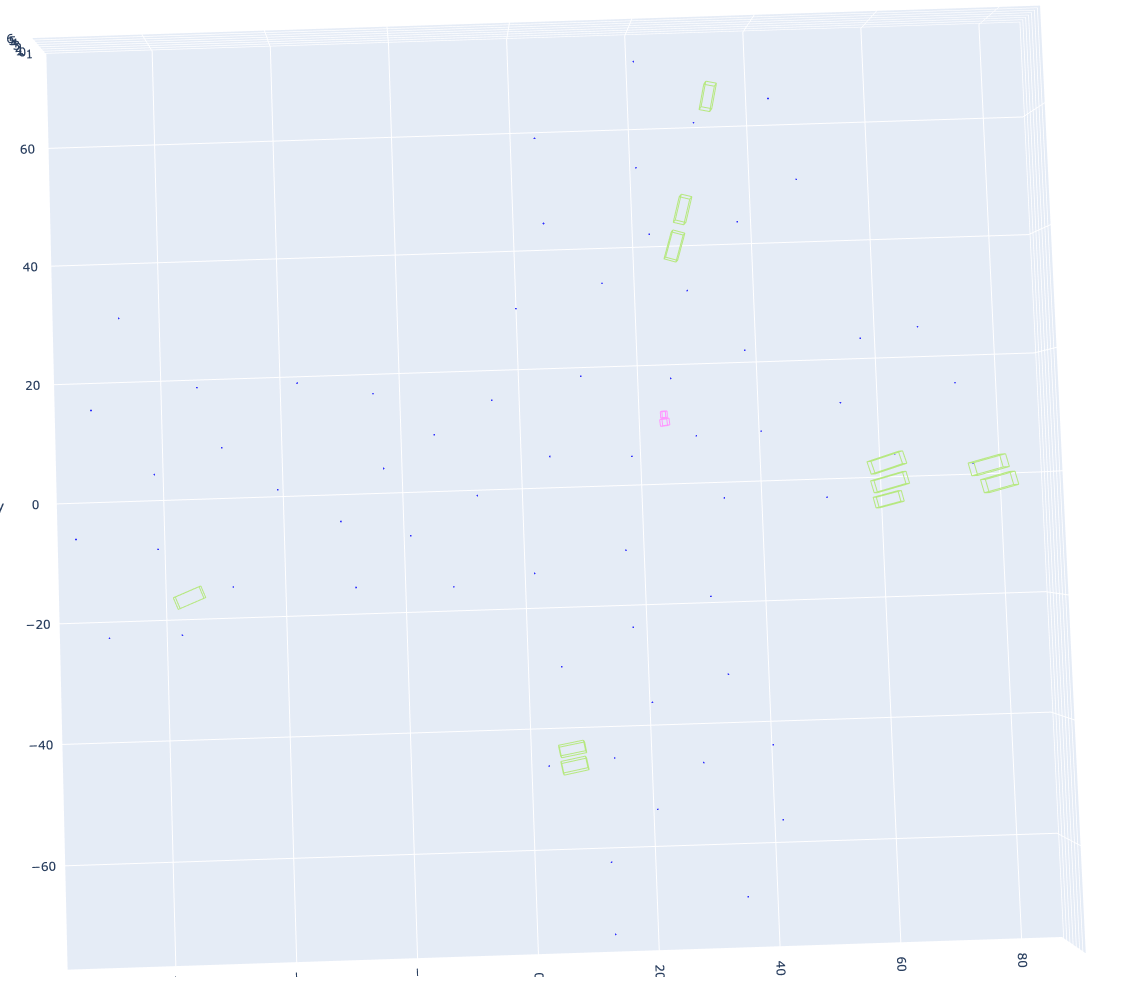
\includegraphics[width=\linewidth]{media/votenet_proposal_points.png}
   \caption{Top view of final 3D space. Blue Points are the final proposal points from VoteNet. Green and Magenta boxes are Ground truth bounding boxes. During training, the final proposal are all lie outside the ground truth bounding boxes. Hence, the voting module cannot learn the correct modules. (Best viewed on screen)}
\label{fig:proposal_points}
\end{figure}

\subsubsection{Results on Front Camera Frustum Point Cloud}
To verify the results of the previous section, we did an extensive exploration in the literature about the experiments involves raw point processing approaches \cite{pointnet, point++, votennet, votenet frustutm, point rcnn} for outdoor datasets \cite{KITTI,  nuscenes, Waymo, a2d2}. interesting work in \cite{point rcnn} in forground background segmentation caught our attention. as a first step, we reproduced the work in \cite{point RCNN} on KITTI dataset \cite{KITTI}. Then, Before reproducing the same experiment on Waymo \ cite{}, we implemented a specific data processing pipeline to make Waymo point cloud identical to KITTI. As KITTI includes annotations only for the objects in teh front camera frustum. we first project the 360-degree LiDAR data onto the image plane and extract the point cloud that lie inside the result- ing frustum. This step reduces the average number on points per scene from $\sim$170k to 16,384. For each scene we randomly subsample 16,384 points, and for scenes with fewer points, we randomly copy the points up to a total of 16,384.

reducing the size of the point cloud make a tremendous boost in the (AP) results of VoteNet when we re-executed the experimetents mentioned in \ref{} on this data setup. due to the small initial input size, the ratio between points inside bounding boxes to the points outside bounding boxes are very large when compared in case of using the 360 point cloud. many of the final proposal points are found inside the ground truth bounding boxes. Thus the voting module was able to learn the correct voting. Figure \ref{fig:votnet_front_camera_results} shows the final results of running two VoteNet architectures on the reduced Waymo point clouds.

\begin{figure}
	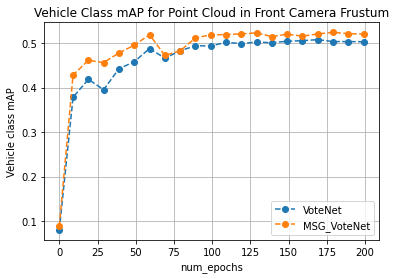
\includegraphics[width=\linewidth]{media/votenet_mAP.png}
   \caption{mAP on Waymo Validation set for Original VoteNet architecture and tuned VoteNet architecture}
\label{fig:votnet_front_camera_results}
\end{figure}


\subsection{Appendix Two Test}

Minkowski Vs Spconv vs Sparse Tensor library


\end{document}
